%%%%%%%%%%%%%%%%%%%%%%% file typeinst.tex %%%%%%%%%%%%%%%%%%%%%%%%%
%
% This is the LaTeX source for the instructions to authors using
% the LaTeX document class 'llncs.cls' for contributions to
% the Lecture Notes in Computer Sciences series.
% http://www.springer.com/lncs       Springer Heidelberg 2006/05/04
%
% It may be used as a template for your own input - copy it
% to a new file with a new name and use it as the basis
% for your article.
%
% NB: the document class 'llncs' has its own and detailed documentation, see
% ftp://ftp.springer.de/data/pubftp/pub/tex/latex/llncs/latex2e/llncsdoc.pdf
%
%%%%%%%%%%%%%%%%%%%%%%%%%%%%%%%%%%%%%%%%%%%%%%%%%%%%%%%%%%%%%%%%%%%


\documentclass[runningheads,a4paper]{llncs}

\usepackage{amssymb}
\setcounter{tocdepth}{3}
\usepackage{graphicx}
\usepackage{amsmath}
\usepackage{url}
\newcommand{\keywords}[1]{\par\addvspace\baselineskip
\noindent\keywordname\enspace\ignorespaces#1}

\begin{document}

\mainmatter  % start of an individual contribution

% first the title is needed
\title{An object-oriented library in JavaScript to build modular and flexible cross-platform evolutionary algorithms}
% Si la has enviado a EvoSTOC, deberías orientarla más en ese
% sentido... "for stochastic optimization", por ejemplo - JJ 
%\title{Lecture Notes in Computer Science:\\Authors' Instructions
%for the Preparation\\of Camera-Ready
%Contributions\\to LNCS/LNAI/LNBI Proceedings}

% a short form should be given in case it is too long for the running head
%\titlerunning{Object-oriented JavaScript library to build cross-platform EA}
% the name(s) of the author(s) follow(s) next
%
% NB: Chinese authors should write their first names(s) in front of
% their surnames. This ensures that the names appear correctly in
% the running heads and the author index.
%

\author{Hidden for double blind review}
%
%%%% modified list of authors for the TOC (add the affiliations)
%
\institute{Hidden for double review}



%
% (feature abused for this document to repeat the title also on left hand pages)

% the affiliations are given next; don't give your e-mail address
% unless you accept that it will be published

%
% NB: a more complex sample for affiliations and the mapping to the
% corresponding authors can be found in the file "llncs.dem"
% (search for the string "\mainmatter" where a contribution starts).
% "llncs.dem" accompanies the document class "llncs.cls".
%

%\toctitle{Lecture Notes in Computer Science}
\maketitle

% Este abstract es todavía el del mío, creo... ¿no lo has cambiado? 
\begin{abstract}
This paper introduces a new distributed evolutionary computation
system that uses the computational capabilities of the web
browser. Using JavaScript in an asynchronous way allows anybody with a web
browser 
to participate in evolutionary experiments with little or none effort. Since, in
this case, computing becomes a social activity and is inherently unpredictable, in this paper we  explore the performance of this kind of virtual computer by solving two simple problems, such as the Royal Road function and a 128-terms equation, and analysing how many machines and evaluations it yields. 
This paper attempts to reproduce results of older papers using modern
browsers and all kind of devices that, nowadays, have JavaScript integrated in the browser, and is a complete rewrite of the code using the popular MooTools library. 
Results show that the system allows the rapid development of evolutionary algorithms, suited for different chromosomes representations and problems, that can be simultaneously executed in many different operating systems and web browsers, sharing the best solutions previously found.
\keywords{Web browser-based computation, Javascript library, asynchronous communication, cross-platform evolutionary algorithms	}
\end{abstract}

% no key words

\section{Introduction and state of the art}
\label{sec:intro}
% no \PARstart
The Javascript language~\cite{javascript} was introduced in Netscape
Navigator in 1995 and quickly adopted by other web browsers. It soon
became a standard proposed by ECMA International in 1997, with the
name of ECMAScript. This interpreted language gives web navigators
(and in fact, many other applications relying on web engines, like
email clients, and lately, since the introduction of {\tt node.js},
any application) the power to perform any computation apart from the
needed to render HTML code. Despite being a language initially
designed to operate over the Document Object Model (DOM) of a web
page, nowadays it has become the most popular language, due mainly to
the fact that, using {\tt node.js}, you need only one language to
create a whole rich internet client-server application.

Javascript offers some good features that can be used for evolutionary computation. First one is related to the interpreter itself, as most applications nowadays run into web browsers; this gives Javascript the opportunity to build web applications that incorporate evolutionary solutions as desktop ones can do. Furthermore, as browsers can be found in most operating systems and devices (from expensive computers to cheap smartphones and tablets), cross-platform interoperability can be yielded with minimum or not effort at all. The second one concerns the intrinsic communicative nature of browsers, i.e., that they are mainly designed to act as clients that send and receives data from web servers. This makes easier the task of running any kind of algorithms in a collaborative way, using many and different hardware and software platforms. 

The communicative aspect of web browsers turn them into the clients of application--level networks (ALNs), which are configured as a set of
clients/servers ({\em servents}). Browser based computation can be then considered as belonging to the so called  {\em volunteer computing}~\cite{sarmenta-bayanihan,hpvc} where volunteer users lend their CPU cycles by means of a downloadable application, and a distributed computation network providing ad hoc computational power is established. SETI@Home is the most well-known ALN, being quite successful \cite{david-seti:home}, it was able to	
create a virtual computer that processed a high amount of
teraflops.  Some companies related to volunteer computing, such as Popular Power and
others ~\cite{Cappello}, did some experimentation with Java based
clients, but none has had commercial success. Volunteer computing has
been previously used in evolutionary computation, using
frameworks such as DREAM \cite{LNCS2439:ID197:pp665}, which includes a
Java-based virtual machine; peer to peer (P2P) examples also exist, as  GOLEM@Home, and G2-P2P \cite{G2-P2P}, in an attempt to avoid bottlenecks produced by the servers.


Usability is also a key feature of these ALN, i.e., its simplicity
of use that turns to be the best way to obtain the participation of as
many users as possible. In this sense, the use of browsers has many advantages. For instance, users do not have to download any special application (even being a simple screen-saver, as is needed in BOINC, the successor to SETI@Home). Furthermore, users, no matter their technical knowledge, are used to deal with browser's interface, i.e, links, forms, layouts, or timeouts. In this sense, using the browser to run this kind of applications do not differ from the way people currently read the newspaper or do the shopping.

In order to create a metacomputer, the existence of an interpreted language in the client like Javascript is only a part of the solution. The other part consists on having an easy, effective way to send and retrieve information from the server in a seamless way. There exist some techniques that allow this kind of communication: AJAX (Asynchronous JavaScript and
XML~\cite{brinzarea2010ajax}), AJAJ (Asynchronous JavaScript and JSON), and {\em remoting} using
applets or embedded objects. Currently, AJAX and AJAJ are widely used since they can be natively executed by web browsers without using external plugins. As can be seen, they only differ in the way the communication is serialized, as AJAX uses XML\cite{goldberg2009xml} to encode both request parameters and data being retrieved, while AJAJ uses JSON. 

Both AJAX and AJAJ work using the same basis: an {\sf XmlHttpRequest} object is created  containing a request to the server, and a reference to a {\em callback} function. 
As the request is being processed, it generates a series of events that can be asynchronously handled by the {\em callback} function, which can also access the data returned by the server.
Both AJAX and AJAJ provide the ways to use the browser for APLs that create distributed computing systems, since this request-response iterative process does not need to interact with humans, as usually happens in any others distributed computing application.
In fact, it even allows to control these APLs from the server with any programming
language. Of course, it can also be combined with other distributed
programming frameworks, as OSGiLiath~\cite{DBLP:journals/soco/Garcia-SanchezGCAG13}, a service oriented architecture for evolutionary algorithms.


This paper presents performance measurements on the jsEO ({\em
  JavaScript Evolving Objects}, pronounce it yi-see-oh) system, which uses PHP 
 (on the server) and JavaScript on the client. Evolutionary computation, being population based method, is suited for this
kind of distributed environment since computation can be distributed among nodes. This can be done both distributing different data portions to every node, or distributing the number of individuals and allowing migration ~\cite{cantu-paz:migration-policies}. In the case of jsEO, the genetic algorithm is carried out  on the clients,
with the server used  for interchange of individuals among
them. A similar approach was used in \cite{agajaj} as a proof of concept, but without establishing an object-oriented hierarchy, so that new evolutionary algorithms, operators, and/or problems could be developed in an easy, and modular way.

In this work, we have performed some experiments in which clients donate
computing power by just loading a web page to find out what kind of
performance we can expect from this kind of setup, from the number of
machines available to the number of evaluations each one of them
usually performs; the results demonstrate this kind of setup is ready to take more
computing-intensive experiments without the need of an expensive server or cluster
setup. 



The rest of the paper is organized as follows: the jsEO library is described next;  methodology and experimental setup can be read  in section \ref{sec:method}, while experiments and results are shown in section 
\ref{sec:exp}; finally, discussion, along with future lines work, are exposed in section \ref{sec:conc}.

\section{The jsEO library}
\label{sec:jseo}
In order to provide a modular, flexible, and object-oriented library, jsEO has been programmed in JavaScript language, making use of the inheritance provided by the MooTools framework (\url{http://mootools,net}). According to pre-existing libraries like EO (written in C++) and JEO (written in Java), jsEO is based on the key-point that any object that can be attached some kind of fitness value is a potential candidate to be evolved. The jsEO library can de downloaded from \url{http://goo.gl/WqTDyM} and it is being developed under the GNU GPLv2 license.

JavaScript's main advantage is that can be executed in most (if not any) web browsers. This allows programs written in this language to be executed in millions of computers, and other devices like smartphones and tablets. JavaScript was mainly designed to operate on the Document Object Model (DOM) browsers generate for every web page they load, thus, content, structure and format style can be dynamically changed while a web page is being visited.

On the other hand, JavaScript's main drawbacks come from the fact that it is interpreted, not compiled, (i.e., slower than desired), it has no access to every resource of the device (e.g. file systems,  memory, or output devices), and that its execution can be stopped by web-browsers if it is consuming too many resources.

Fig.~\ref{fig:jsEO-class-diagram} shows the class diagram of the library. As can be seen, there exist some abstract class which define the general structure of any evolutionary solution to a given problem. Main class is \textit{jsEO}, which represents any object to which a fitness can be assigned, and, consequently, that can be compared with any other. Starting from \textit{jsEO} class, class \textit{jsEOIndividual} can be derived representing any object that contains a chromosome and, therefore, can be evaluated by means of a fitness function. A \textit{jsEOPopulation} is an aggregation of individuals; it can be used to add, replace or remove individuals, can be sorted, and can be also asked to return a subset of individuals.

In order to build algorithms, operators have to be defined. Any operator inherits from \textit{jsEOOperator}, gets a population as input parameter, and returns a population; thus, it is designed for both operators affecting only one individual and operators acting over a whole population.

Once defined the initial core set of abstract classes (except for \textit{jsEOPopulation}), concrete classes has been derived in order to implement the Standard Genetic Algorithm (\textit{jsEOGA}). This algorithm uses the tournament selector to create sub-populations to which mutator and crossover operators can be applied so that they are made to evolve.

Two special operators have been implemented in order to solve problems in a cooperative environment. The first one, \textit{jsEOSendIndividual}, is intended to send the chromosome and fitness of the best individual to a server where it is stored in case it is best solution found up to the moment. The second one, \textit{jsEOGetIndividual}, makes exactly the opposite: it asks the server for the individual being stored and includes it as a new individual in the population. The communication between the client and the server is done using AJAX technology, and made in an asynchronous way when sending the individual to the server, but in a synchronous way in the case of the \textit{jsEOGetIndividual}. Currently, the server has been programmed in PHP and stores data in a row file, in order to ease the implementation on anyone's server. Every synchronized problem executed with jsEO has to be assigned a unique identifier so that the server can discriminate every task when receiving and sending individuals to the clients.

\begin{figure}
\centering
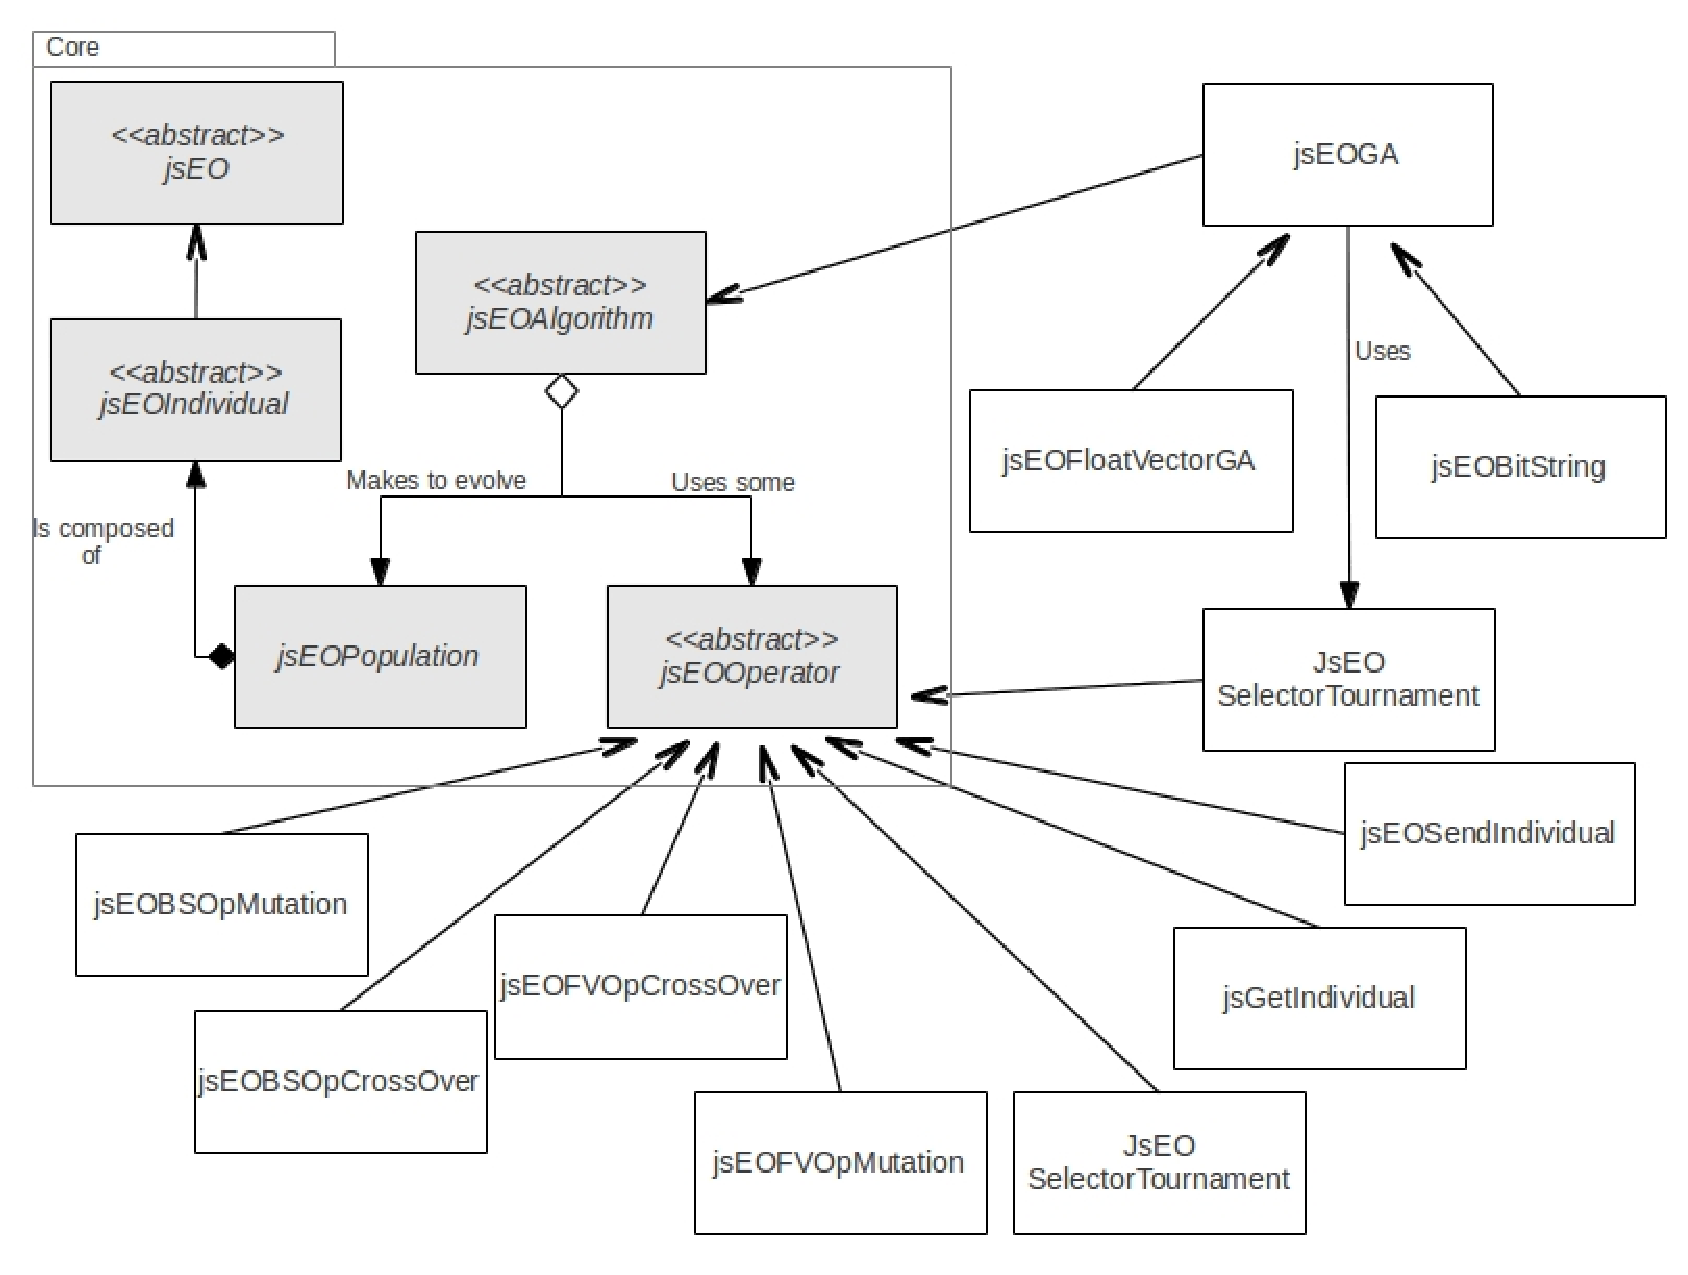
\includegraphics[height=8cm]{class-diagram}
\caption{Class diagram of jsEO. The core package includes some abstract classes (\textit{jsEO, jsEOIndividual}, \textit{jsEOAlgorithm}, and \textit{jsEOOperator}) that make easier to develop new evolutionary algorithms by means of inheritance.}
\label{fig:jsEO-class-diagram}
\end{figure}


\section{Methodology and Experimental Setup}
\label{sec:method}
The experiments designed to test jsEO include two problems, being the first the 256-bit Royal Road function, while the second is solving a 128-terms linear equation. In others words, the first one is related to a bit-string chromosome problem, while the second deals with vector of floats. Both problems have been executed as synchronized tasks, and are available at \url{http://goo.gl/3lJj8Q}. Currently, synchronizing is quite constrained since it is done by means of AJAX connections to a server, without allowing to perform requests from pages hosted on a different one. 

Asking for collaboration to run the experiments was done publishing some messages in social nets as Facebook and Twitter, as well as sending an email to a group of about 70 computer-scientist professionals. The user who wanted to participate in the experiments only had to load in his/her browser a web file containing a brief description of the problem and the Javascript library, and the chosen problem was automatically executed. Users were able to select the problem they wanted to execute, to execute it as many time as desired, to change the problem at any moment, and, of course, to stop the execution by closing the browser or loading a new web page.

In order to execute every problem, two new classes were derived from class \textit{jsEOGA}, the first one to deal with bit-string chromosomes, the second one to make evolve vector of floats. The \textit{jsEOGA} is a steady state algorithm, with rank-based selection, and elimination of the worst individuals after joining the current population of every generation with the new individuals created by means of operators. The algorithm stopped after a given number of generations (table~\ref{tb:params} shows the parameters used), and incorporated operators for crossover and mutation. In the case of real problem, mutation consist on changing values for new random ones. After every generation, best individual was sent to the server. On the other hand, requesting an individual to the server was done randomly according to the application rate of the corresponding \textit{jsEOGetIndividual} operator. Finally, two different evaluation functions were used, one per problem. In the case of 256-bit Royal Road function, the fitness corresponds to the number of "1111" or "0000" sequences found in the 256-length bit-string. In the case of 128-terms equation, the fitness was the inverse of the value obtained when evaluating a linear equation with 128 real values in the range $(-10,10)$ composing every chromosome. The exact solution is the one containing the terms that can be downloaded from \url{http://goo.gl/jI0Wt0}.
	
Since both problems have been executed in a synchronous way, the best solution can be found in the server, but also in many clients as this individual is sent to the browser as soon as the \textit{jsEOGetInvididual} operator is selected to operate.



\begin{table}
\caption{Parameters used to run the experiments, as in{\cite{agajaj}}}
\begin{center}
\begin{tabular}{l@{\quad}rl}
\hline
\multicolumn{1}{l}{\rule{0pt}{12pt}
                   Parameter}&\multicolumn{2}{l}{Value}\\[2pt]
\hline\rule{0pt}{12pt}
Population size & 500 & \\
Tournament size & 2 & \\
Operator crossover's rate & 0.73 & \\
Operator mutation's rate & 0.18 & \\
Operator requesting individual's rate & 0.09 & \\
Number of genes affected by mutation & $1\%$ &\\
Individuals replaced in every generation & $50\%$ & \\
Range for new random real values && \\
(only for the 128-term equation problem) & $(-10,10)$ & \\[2pt]
\hline

\end{tabular}
\label{tb:params}
\end{center}
\end{table}

  	




\section{Experimental results}
\label{sec:exp}

After two days of volunteers executing the algorithms, some results can be drawn gathering data from the web server's log file (in this case, Apache log). The log file has been analysed using the free version of WebLog Expert application\footnote{WebLog Expert can be obtained from \url{http://www.weblogexpert.com/}}, and the well-known Webalizer application\footnote{Webalize can be obtained from \url{http://www.webalizer.com}}.

From a potential target of users of more than 500 people, the 128-terms equation has been executed 304 times by 231 different visitors, while the 256-bit Royal Road function has been executed 359 times by 279 visitors. Most of this visits (i.e., executions) were done along a period of approximately 24 hours, but no references about time consumed by every execution have been registered. The algorithms have been executed in up to 128 different combinations of web browser and operating system, any of them in many different versions. As shown in figures \ref{fig:browsers} and \ref{fig:operating-systems}, Web browser include Safari, Firefox, Chrome, Internet Explorer, and native browsers for smartphones and tablets; while operating systems include Windows, Linux, MacOS, and Android.

\begin{figure}
\centering
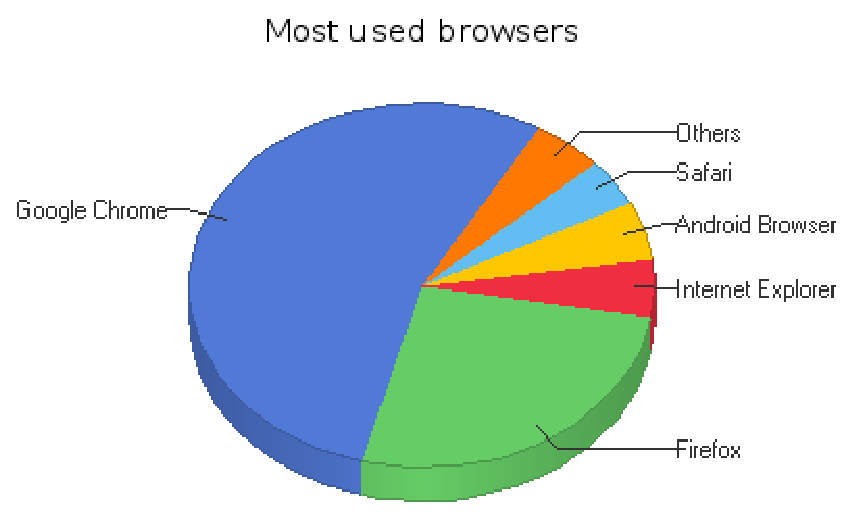
\includegraphics[height=5cm]{Most_Used_Browsers}
\caption{Summary of browsers used to run the experiments. For any of the browsers, many different versions have been used. For instance, up to 4 different versions of Internet Explorer were found.}
\label{fig:browsers}
\end{figure}


\begin{figure}
\centering
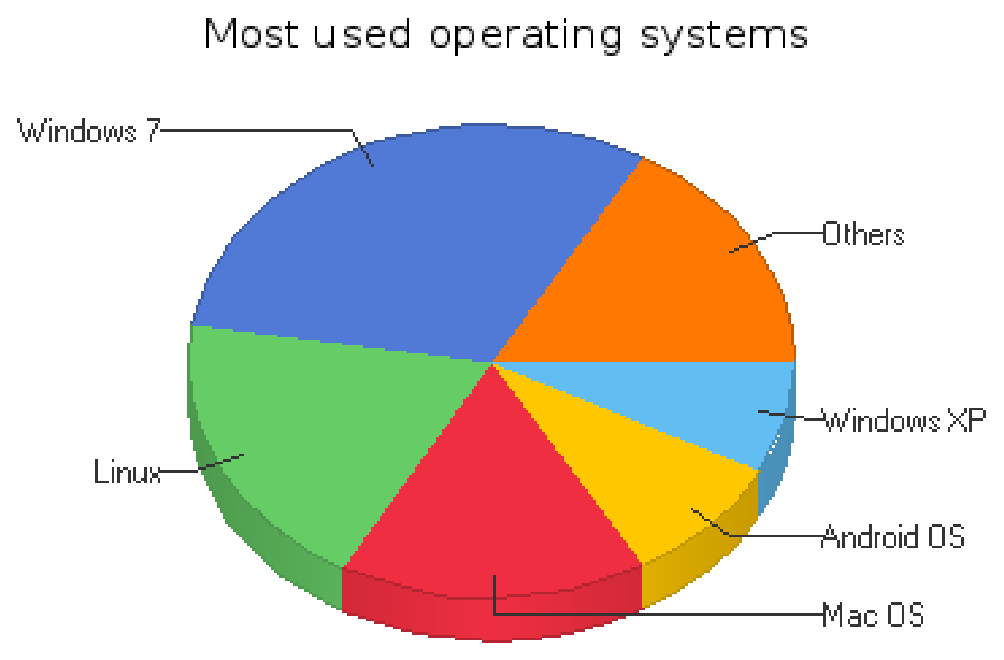
\includegraphics[height=5cm]{Most_Used_Operating_Systems}
\caption{Set of operating systems that have been used by users visiting the pages containing the experiments. The figures corresponding to Windows include 8 different versions, including the one for phones.
}
\label{fig:operating-systems}
\end{figure}

As can be seen in table~\ref{tb:params}, population was composed by $500$ individuals, and $50\%$ were replaced in every generation, this means that in every execution $13,000$ individuals were evaluated. Consequently, the currently available solutions in the server have been found after $3,952,000$ evaluations in the case of the 128-terms equation, and $4,667,000$ evaluations for the 256-bit Royal Road function. The solution found for the bit-string problems is composed by 176 characters "0", and 80 characters "1", being  its fitness 232. For the real codified problem, the solution yields a fitness of $300,909.09$, which corresponds to a value of $3.32E-06$ when evaluating the equation being solved.

\section{Conclusions, discussion and future work}
\label{sec:conc}

In this paper we have proved that, 
without an expensive or far-fetched setup, volunteer computation can achieve high
performance, equivalent, at most, to several computers of average
performance. The code used to perform the experiment is publicly
available and is modular so that creating different experiments is
just a matter of writing a new JavaScript fitness function and tuning
the GA parameters accordingly. 

The experiments have proved that there is a good amount of
computational power that can be easily tapped and used for
evolutionary computation experiments, however, the nature of jsEO
constrains also the way users donate computing power, as well as the
number of clients available for an experiment. In this paper we have
found some figures, which will undoubtedly vary for other experiments;
however, the general shape of the curves will probably be the same,
following a very steep decrease from the maximum values obtained. 

The GA, being asynchronous, faces some problems that have not been
tackled in this paper. What is the best approach to preserve
diversity? To generate a new population in each client, and receive
immigrants as soon as possible, which are incorporated into the
population? Or is it better to create new client populations based on
existing populations? What is really the algorithmic contribution of
new clients? These issues will be explored as future work. 
We will also measure the limits of this technology, and test
the impact of servers of varying performance and workload on overall
performance. Eventually, we will also try to perform a {\em sneaky}
experiment, to check what kind of performance can be expected in that
kind of setups. 

\section*{Acknowledgements}

Hidden for double-blind review

\bibliographystyle{unsrt}
\bibliography{europar2007,GA-general,geneura,ror-js,volunteer,web-ajax-xml-javascript}


% that's all folks
\end{document}
